\documentclass{article}
\usepackage{listings}
\usepackage{amsmath}
\usepackage{fullpage}
\usepackage{tabularx}
\usepackage{graphicx}
\usepackage{tikz}
\usetikzlibrary{shapes.geometric, arrows}
\usepackage{cite}
\usepackage{hyperref}
\usepackage{float}
\begin{document}
\lstset{language=python, tabsize=4}
\title{Node mapping}
\author{Yuchen Hou \and Larry Holder}
\maketitle

\begin{abstract}
	We present node mapping, a technique created for link attribute prediction 
	tasks, powered by neural networks.
	This technique builds a neural net model, which learns to map every node in 
	a graph to a node vector of real numbers and learns to predict the target 
	link attribute using these node vectors.
	Every node vector contains information about the node related to the
	prediction task.
	The main idea is to convert nodes (categorical variables) to vectors 
	(numerical variables), as neural nets can directly handle only numerical 
	variables.
\end{abstract}

\section{Introduction}

\subsection{Background}
We have seen the wide spread success of neural networks since 2010, as they are 
becoming state-of-the-art models in a growing number of application domains of 
machine learning, (e.g., speech recognition\cite{hannun2014deep}, image 
recognition\cite{simonyan2014very}, and natural language 
processing\cite{yao2013recurrent}).
These neural net models not only achieved higher prediction accuracy than 
traditional models, but also require much less domain knowledge and engineering.
In 2016, Google AlphaGo AI - powered by neural net and Monte Carlo tree search 
- defeated go champion Lee Sedol, demonstrated how a statistical approach can 
complement logical approaches in solving challenging 
problems\cite{silver2016mastering}.
Specifically, in a game like go with simple rules but too many possible 
configurations to explore, neural net models achieve good results with 
reasonable computing resources, which are easily exhausted by algorithms solely 
powered by search.

\subsection{Motivation}
As neural nets have demonstrated their power in many domains, we naturally 
wonder if we can apply them in prediction tasks in graph mining domain, and 
what kind of techniques are helpful in using their power.
There are existing techniques with promising results already.
Two earlier attempts were graph neural nets and relational neural 
nets\cite{scarselli2009graph}, where neural nets are incorporated into a 
traditional iterative graph information propagation approach.
A later attempt was deep walk\cite{perozzi2014deepwalk}, where a graph is 
reduced to a natural language corpus so that existing neural net models 
designed for natural language processing can handle the graph.
We find these techniques complex, indirect and unable to fully use rich graph 
information in real applications, e.g. making recommendations for social 
network users based on user activities like messaging friends, commenting 
articles, and rating movies.
However, these attempts all include an essential step of applying neural net in 
graphs: converting graph to numerical variables.
This step is essential in other application domains as well, because neural 
nets cannot directly handle non-numerical variables.

\subsection{Goal}
We want to create a technique to predict link attributes in a graph using a 
neural net model. The graph can have any topology and its links can have any 
number of numerical(including boolean) attributes. The technique should build a 
neural net model, which learns to represent the graph in a meaningful way and 
to predict the target link attribute using the representation it learns.

\section{Observations and approach}
In order to understand how a neural net can handle prediction tasks in graphs, 
we take an overview on 3 types entities in these 3 domains and in graph mining. 
\autoref{tab:domains} provides a summary of these entities, their 
representations in neural nets and inter-entity relation examples in these 
domains.
\begin{table}[H]
	\centering
	\begin{tabularx}{\textwidth}{ |c|c|c|X| }
		\hline domain & entity & representation & relations to other entities 
		\\ 
		\hline image recognition & image & 2D light intensity array & NA \\ 
		\hline speech recognition & utterance/spectrogram & 2D sound intensity 
		array & NA \\ 
		\hline natural language & word & word vector & relations to other words 
		\\ 
		\hline graph & movie & node vector & directed by director, etc \\ 
		\hline graph & user & node vector & rate movies, etc \\
		\hline
	\end{tabularx}
	\caption{A summary of various types of entities, their numerical 
	representations and inter-entity relations in different domains: images and 
	utterances can be directly represented by 2D numerical arrays, but have no 
	strong relations to other images or utterances; words and various types of 
	nodes in graphs can represented by 1D numerical arrays(which will be 
	introduced below), and have strong relations to other words and nodes. 
	Notice that the representations for all the entities are numerical arrays, 
	because neural nets rely on neurons' activations and communications, which 
	are both numerical.}
	\label{tab:domains}
\end{table}

\subsection{Entity representations in different domains}
In \autoref{tab:domains}, the entities listed in the lower rows have increasing 
representation complexities. Images and utterances(spectrograms) can be 
naturally represent as 2D numerical arrays, which makes them easy for neural 
net to process. Words are categorical variables and consequently harder, but 
they can be mapped to 1D numerical arrays (i.e. word vectors) by word2vec 
technique \cite{mikolov2013efficient} so neural nets can still process them.

\subsection{Learning word vectors}
Interestingly, it turns out neural net itself has the capability to do the 
mapping.
In word2vec, a neural net learns to map every word to a vector without any 
domain knowledge. In a corpus, every word is described/defined only by related 
words in its context, although relations between the words are implicit. 
Nonetheless, the neural net can learn from word co-occurrences and map words 
accordingly such that the relations between words are preserved in the vector 
space \cite{mikolov2013distributed}.

\subsection{Learning node vectors}
If we compare language data and graph data, we can immediately realize they 
have many similarities, shown in \autoref{tab:wordVSnode}.
\begin{table}[H]
	\centering
	\begin{tabularx}{\textwidth}{ |X|X|X| } \hline
		aspect  & natural language processing & graph mining \\ \hline
		dataset & corpus & graph \\ \hline
		basic entities & words & nodes \\ \hline
		entity collection & vocabulary & node set \\ \hline
		relations & co-occurrences (implicit) & links (explicit) \\ \hline
		representation & word vectors & node vectors \\ \hline
	\end{tabularx}
	\caption{A comparison of language data and graph data from 
		several aspects: these similarities suggest a neural net might be able 
		to map nodes to node vectors just like mapping words to word vectors.}
	\label{tab:wordVSnode}
\end{table}
Apparently, mapping node to node vectors should be more direct than mapping 
word to word vectors, because the relations between nodes are explicit(i.e., 
link and link attributes), while relations between words are implicit(i.e., 
word co-occurrences). In a social network example, the rating a movie received 
from a user explicitly tells us how much the user likes that movie; the number 
of messages a user sends to another user explicitly tells us how close they are 
connected. In a corpus example, the co-occurrences of words [the, quick, brown, 
fox, jumps, over] implicitly suggest these words may be related but do not tell 
us what their relations are. This means the neural net should be able to learn 
node mapping supervised by the link attributes in a more direct way than it 
learns word mapping supervised by word co-occurrences.

\subsection{Application scenario}

\subsubsection{The dataset}
\begin{table}[H]
	\centering
	\begin{tabularx}{0.5\textwidth}{|c|X| }  \hline
		nodeID & labels \\ \hline
		0 & [ture, false, false... true] \\ \hline
		1 & [ture, true, false... false] \\ \hline
		2 & [false, false, false... true] \\ \hline
		... & ... \\ \hline
		n & [ture, false, true... true] \\ \hline
	\end{tabularx}
	\caption{The node set: a node can have a number of labels.}
\end{table}
\begin{table}[H]
	\centering
	\begin{tabularx}{0.5\textwidth}{|X|X|}  \hline
		sourceID & destinationID \\ \hline
		0 & 4355 \\ \hline
		0 & 987876 \\ \hline
		2 & 324 \\ \hline
		... & ... \\ \hline
		n & x \\ \hline
	\end{tabularx}
	\caption{The link set: a link has no attributes}
\end{table}
\begin{itemize}
	\item dataset: graph = (nodes, links)
	\item link attribute: none
	\item node attribute: labels(list of booleans)
\end{itemize}

\subsubsection{Prediction task: node attribute prediction}
\begin{enumerate}
	\item input: X = node, node in nodes
	\item output: Y = [y[0], y[1], y[2] ... y[n-1]], y[i] in [true, false]
\end{enumerate}

\subsection{Implementation}

\subsubsection{Node mapping stage}
\begin{itemize}
	\item model: skip-gram model
	\item node sequence generation: sampled random walks on the graph
	\item weights update: weights in all layers
	\item learning outcome: node vectors stored in weights in mapping layer
\end{itemize}
\subsubsection{Label prediction stage}
\begin{itemize}
	\item model: adjust output layer size to label set size
	\item weights update: weights in output layer only
\end{itemize}
\begin{figure}[H]
	\centering
	\newcommand{\layersep}{2.5cm}
	\newcommand{\vocabularySize}{8}
	\newcommand{\mappingSize}{4}
	\newcommand{\labelSetSize}{2}
	\begin{tikzpicture}[shorten >=1pt,->,draw=black!50, node distance=\layersep]
	\tikzstyle{every pin edge}=[<-,shorten <=1pt]
	\tikzstyle{neuron}=[circle,fill=black!25,minimum size=17pt,inner sep=0pt]
	\tikzstyle{input neuron}=[neuron, fill=green!50];
	\tikzstyle{output neuron}=[neuron, fill=red!50];
	\tikzstyle{hidden neuron}=[neuron, fill=blue!50];
	\tikzstyle{annot} = [text width=4em, text centered]
	
	% Draw the input layer
	\foreach \name / \y in {1,...,\vocabularySize}
	% This is the same as writing \foreach \name / \y in {1/1,2/2,3/3,4/4}
	\node[input neuron, pin=left:$ node_\y $] (I-\name) at (0,-\y) {};
	
	% Draw the hidden layer
	\foreach \name / \y in {1,...,\mappingSize}
	\path[yshift=-2cm]
	node[hidden neuron] (H-\name) at (\layersep,-\y) {};
	
	% Draw the output layer
	\foreach \name / \y in {1,...,\labelSetSize}
	\node[output neuron, pin={[pin edge={->}]right:$ label_\y $}] (O-\name) at 
	(2*\layersep,-\y-3) {};
	
	% Connect the input layer with the hidden layer
	\foreach \source in {1,...,\vocabularySize}
	\foreach \dest in {1,...,\mappingSize}
	\path (I-\source) edge (H-\dest);
	
	% Connect the hidden layer with the output layer
	\foreach \source in {1,...,\mappingSize}
	\foreach \dest in {1,...,\labelSetSize}
	\path (H-\source) edge (O-\dest);
	
	% Annotate the layers
	\node[annot,above of=H-2] {mapping layer};
	\node[annot,above of=I-2] {input layer};
	\node[annot,above of=O-2] {output layer};
	\end{tikzpicture}
	\caption{The label prediction model with node set size 8, mapping size 4 
	and label set size 2: learning label prediction.}
	\label{fig:label}
\end{figure}

\subsection{Strengths of this approach}

\subsubsection{Representing nodes as node vectors}
\begin{table}[H]
	\centering
	\begin{tabularx}{0.5\textwidth}{ |c|X|X| } \hline
		aspect  & node & link \\ \hline
		complexity & high & low \\ \hline
		observability & low & high \\ \hline
		example & user & activities \\ \hline
	\end{tabularx}
	\caption{A comparison of node and link with respect to their complexity and 
	attribute observability: what one does tells us what kind of person he is.}
	\label{tab:nodesVSlinks}
\end{table}

\subsubsection{Online learning}
\begin{itemize}
	\item low memory requirement
	\item incremental model construction
	\item suitable for streaming graph
\end{itemize}

\subsection{Weaknesses of this approach}

\subsubsection{Node sequence generation}
\begin{enumerate}
	\item remote nodes in a deep walk is not strongly related to the root
	\item skip-gram's indifference to important node ordering
	\item power law node frequency distributions
\end{enumerate}

\subsubsection{Unable to use rich attributes in graph}
\begin{itemize}
	\item nodes and links have attributes
	\item attributes can provide more information than topology
\end{itemize}

\begin{figure}[H]
	\centering
	\newcommand{\layersep}{8}
	\newcommand{\vocabularySize}{3}
	\newcommand{\mappingSize}{5}
	\begin{tikzpicture}[shorten >=1pt,->,draw=black!50, node distance=\layersep]
	\tikzstyle{every pin edge}=[<-,shorten <=1pt]
	\tikzstyle{neuron}=[circle, draw, minimum size=20]
	\tikzstyle{input neuron}=[neuron];
	\tikzstyle{output neuron}=[neuron];
	\tikzstyle{hidden neuron}=[neuron];
	\tikzstyle{annot} = [text width=4em, text centered]
	
	% Draw the input layer
	\foreach \name / \y in {1,...,\vocabularySize}
	\node[input neuron] (I-\name) at (0,-2*\y) {$ user_\name $};
	
	% Draw the hidden layer
	\foreach \name / \y in {1,...,\mappingSize}
	\path[yshift=2cm]
	node[hidden neuron] (H-\name) at (\layersep,-2*\y) {$ movie_\name $};
	
	% Connect the input layer with the hidden layer
	\foreach \source in {1,...,\vocabularySize}
	\foreach \dest in {1,...,\mappingSize}
	\path (I-\source) edge (H-\dest);
	\end{tikzpicture}
	
	\caption{The weakness of solely relying on topology and ignoring other rich 
	attributes: unable to discriminate nodes.}
	\label{fig:weakness}
\end{figure}

\section{Node mapping for graphs with rich attributes}

\subsection{Advanced features/strengths}
\begin{enumerate}
	\item comprehensive learning: exploiting rich node and link attributes
	\item multi-task prediction: learn to predict any node or link attribute
\end{enumerate}

\subsection{Application scenario}

\subsubsection{The dataset}
\begin{table}[H]
	\centering
	\begin{tabularx}{0.5\textwidth}{|X|X| }  \hline
		userID & french \\ \hline
		0 & false \\ \hline
		1 & false \\ \hline
		2 & true \\ \hline
		... & ... \\ \hline
		n & false \\ \hline
	\end{tabularx}
	\caption{The node set: a user has 1 boolean attribute - french}
	\label{tab:user}
\end{table}
\begin{table}[H]
	\centering
	\begin{tabularx}{0.5\textwidth}{|X|X|X| }  \hline
		userID & movieID & rating \\ \hline
		0 & 4355 & 4 \\ \hline
		0 & 987876 & 7 \\ \hline
		2 & 324 & 2 \\ \hline
		... & ... & ... \\ \hline
		n & x & 9 \\ \hline
	\end{tabularx}
	\caption{The link set: a link has 1 numerical attribute - rating}
	\label{tab:rating}
\end{table}
\begin{itemize}
	\item dataset: graph = (\{users and movies\}, ratings)
	\item movie attribute: none
	\item user attribute: french(boolean)
	\item link attribute: rating(numerical)
\end{itemize}

\subsubsection{Prediction task: node attribute prediction}
\begin{enumerate}
	\item input: X = user, user in users
	\item output: Y = french, french in [true, false]
\end{enumerate}

\subsubsection{Prediction task: link attribute prediction}
\begin{enumerate}
	\item input: X = (user, movie), user in users, movie in movies
	\item output: Y = rating, rating in range(1, 10)
\end{enumerate}

\subsection{Observations and the approach}
\begin{enumerate}
	\item french: information about the user
	\item rating: information about the user and the movie
	\item learning: supervised by both attributes
\end{enumerate}

\subsection{Implementation}

\subsubsection{Multi-task model}
\begin{figure}[H]
	\centering
	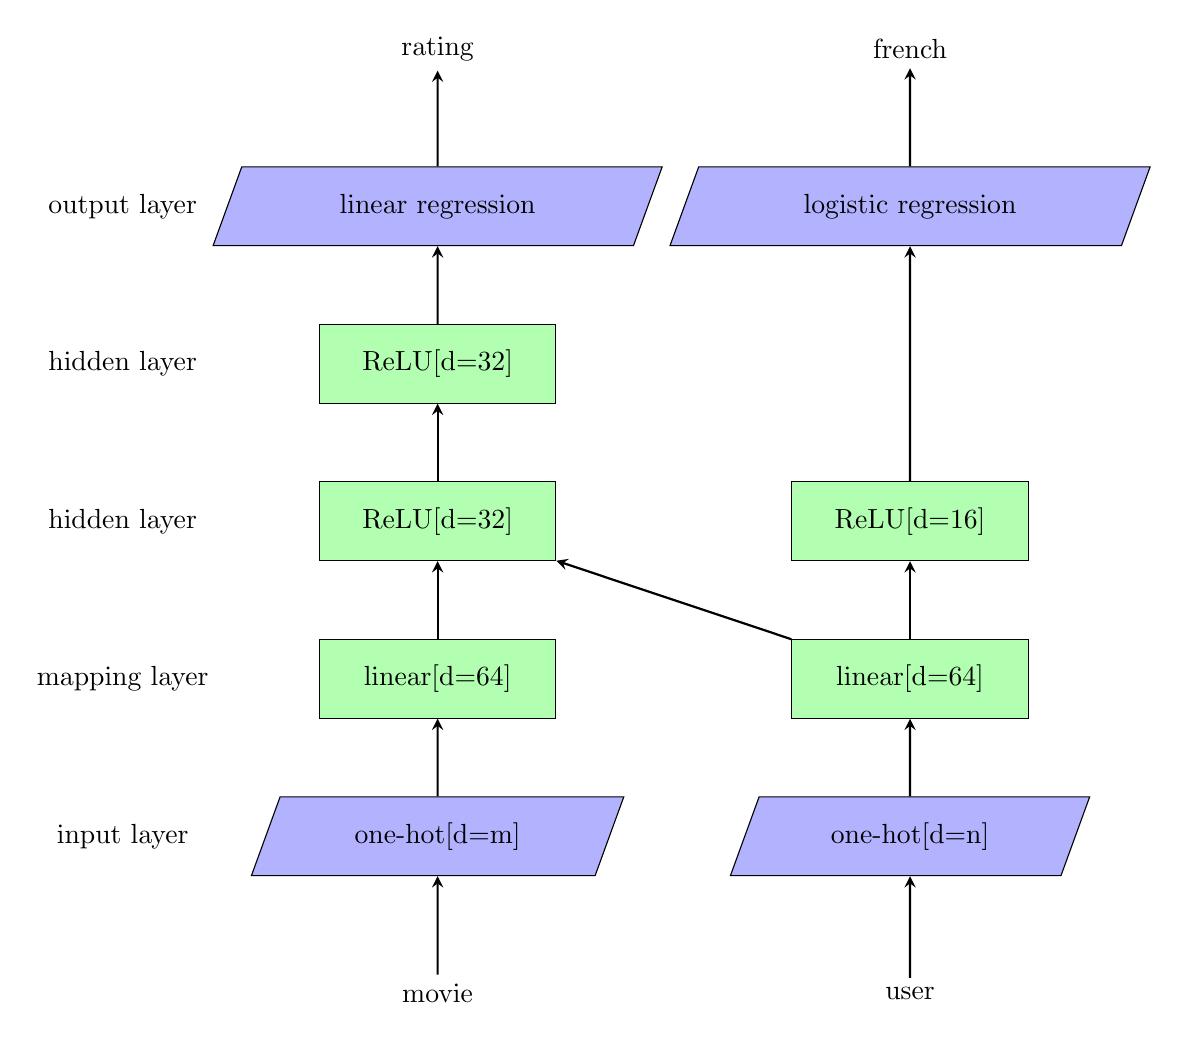
\begin{tikzpicture}[node distance=2cm]
	\tikzstyle{io} = [trapezium, trapezium left angle=70, trapezium right 
	angle=110, minimum width=0cm, minimum height=1cm, text centered, 
	draw=black, fill=blue!30]
	\tikzstyle{process} = [rectangle, minimum width=3cm, minimum height=1cm, 
	text centered, draw=black, fill=green!30]
	\tikzstyle{arrow} = [thick,->,>=stealth]
	\node (linearRegression) [io] {linear regression};
	\node (logisticRegression) [io, right of=linearRegression, xshift=4cm] 
	{logistic regression};
	\node (relu1) [process, below of=logisticRegression, yshift=-2cm] 
	{ReLU[d=16]};
	\node (relu2) [process, below of=linearRegression] {ReLU[d=32]};
	\node (relu3) [process, below of=relu2] {ReLU[d=32]};
	\node (linear1) [process, below of=relu1] {linear[d=64]};
	\node (linear2) [process, below of=relu3] {linear[d=64]};
	\node (oneHot2) [io, below of=linear1] {one-hot[d=n]};
	\node (oneHot1) [io, below of=linear2] {one-hot[d=m]};
	\node (rating) [above of=linearRegression] {rating};
	\node (french) [above of=logisticRegression] {french};
	\node (output) [left of=linearRegression, xshift=-2cm] {output layer};
	\node (hidden2) [below of=output] {hidden layer};
	\node (hidden1) [below of=hidden2] {hidden layer};
	\node (mapping) [below of=hidden1] {mapping layer};
	\node (input) [below of=mapping] {input layer};
	\node (movie) [below of=oneHot1] {movie};
	\node (user) [below of=oneHot2] {user};
	\draw [arrow] (movie) -- (oneHot1);
	\draw [arrow] (user) -- (oneHot2);
	\draw [arrow] (oneHot2) -- (linear1);
	\draw [arrow] (oneHot1) -- (linear2);
	\draw [arrow] (linear1) -- (relu1);
	\draw [arrow] (linear1) -- (relu3);
	\draw [arrow] (linear2) -- (relu3);
	\draw [arrow] (relu3) -- (relu2);
	\draw [arrow] (relu1) -- (logisticRegression);
	\draw [arrow] (relu2) -- (linearRegression);
	\draw [arrow] (linearRegression) -- (rating);
	\draw [arrow] (logisticRegression) -- (french);
	\end{tikzpicture}	
	\caption{The multi-task prediction model with movie set size m, user set 
	size n, mapping size 64: learning rating and french attribute prediction.}
	\label{fig:multiTask}
\end{figure}
\begin{itemize}
	\item mapping layer with linear units: $ y = f(x) = w x $
	\item hidden layers with ReLU(rectified linear units): $ y = f(x) = max(0, 
	w x) $
	\item output layer with linear regression unit: $ y = f(x) = w x $
	\item output layer with logistic regression unit: $ y = f(x) = \frac{1}{1 + 
	exp(-w x)} $
	\item hinge loss for logistic regression: $ loss = l(t, y) = max(0, 1 - ty) 
	$
	\item squared error for linear regression: $ loss = l(t, y) = (t - y)^2 $
\end{itemize}

\section{Conclusions}
This technique has the following strengths:
\begin{enumerate}
	\item low complexity: it is simple and scalable
	\item high flexibility: it can learn from and predict rich node and link 
	attributes
	\item high efficiency: it is very streamlined online learning without any 
	expensive graph operations(not even neighbor node lookup or random walk)
\end{enumerate}
and the following weaknesses:
\begin{enumerate}
	\item unable to handle non-numerical attributes: e.g., a message from user 
	A to user B (a link from A to B) or an article (a node) contain texts 
	(string attributes), which this technique cannot directly handle
\end{enumerate}
\begin{itemize}
	\item node mapping: neural net approach for learning vector 
	representations of nodes
	\item online learning: good for streaming graph
	\item node mapping for graphs with rich attributes: low complexity, 
	comprehensive learning and multi-task prediction
\end{itemize}
\begin{figure}[H]
	\centering
	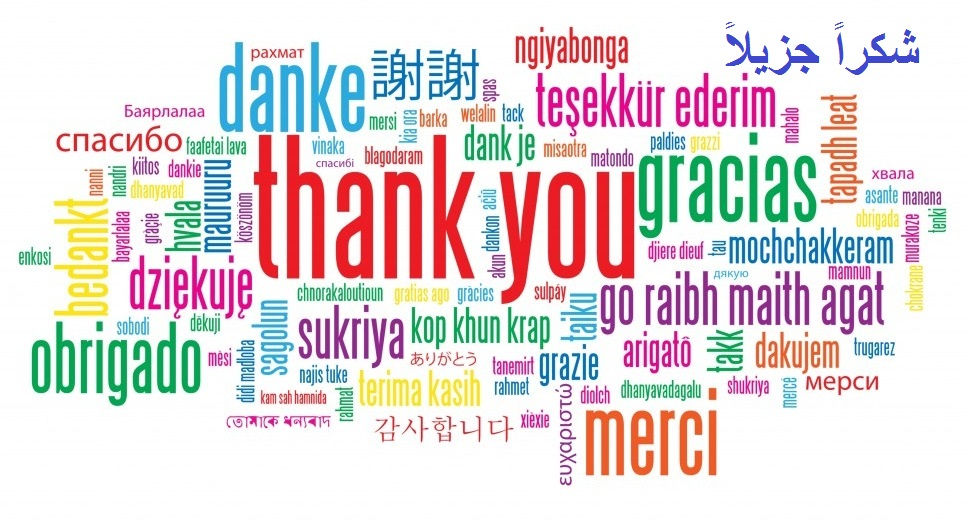
\includegraphics[width=\linewidth]{Thank-you-word-cloud}
	\caption{ 
	\href{https://commons.wikimedia.org/wiki/File:Spectrogram-19thC.png}{Thank 
	you word cloud}(Aquegg / Wikimedia Commons / Attribution-Share Alike 4.0 
	International)}
	\label{fig:Thank-you-word-cloud}
\end{figure}

\bibliographystyle{acm}
\bibliography{references}

\end{document}
